% !TeX root = ../thuthesis-example.tex
\chapter{Design}\label{chapter-3}
This section introduces the overall design of the \Project system (Figure \ref{fig:main-design-figure}), and gives an overview of all its components. To better illustrate the interplay among the various components of the system, we added numbers 1-7 on the figure below. The numbers show the path that a request takes from the user through the system. We discuss the element corresponding to each number below.

\begin{figure}[H]
    \centering
    \fbox{
    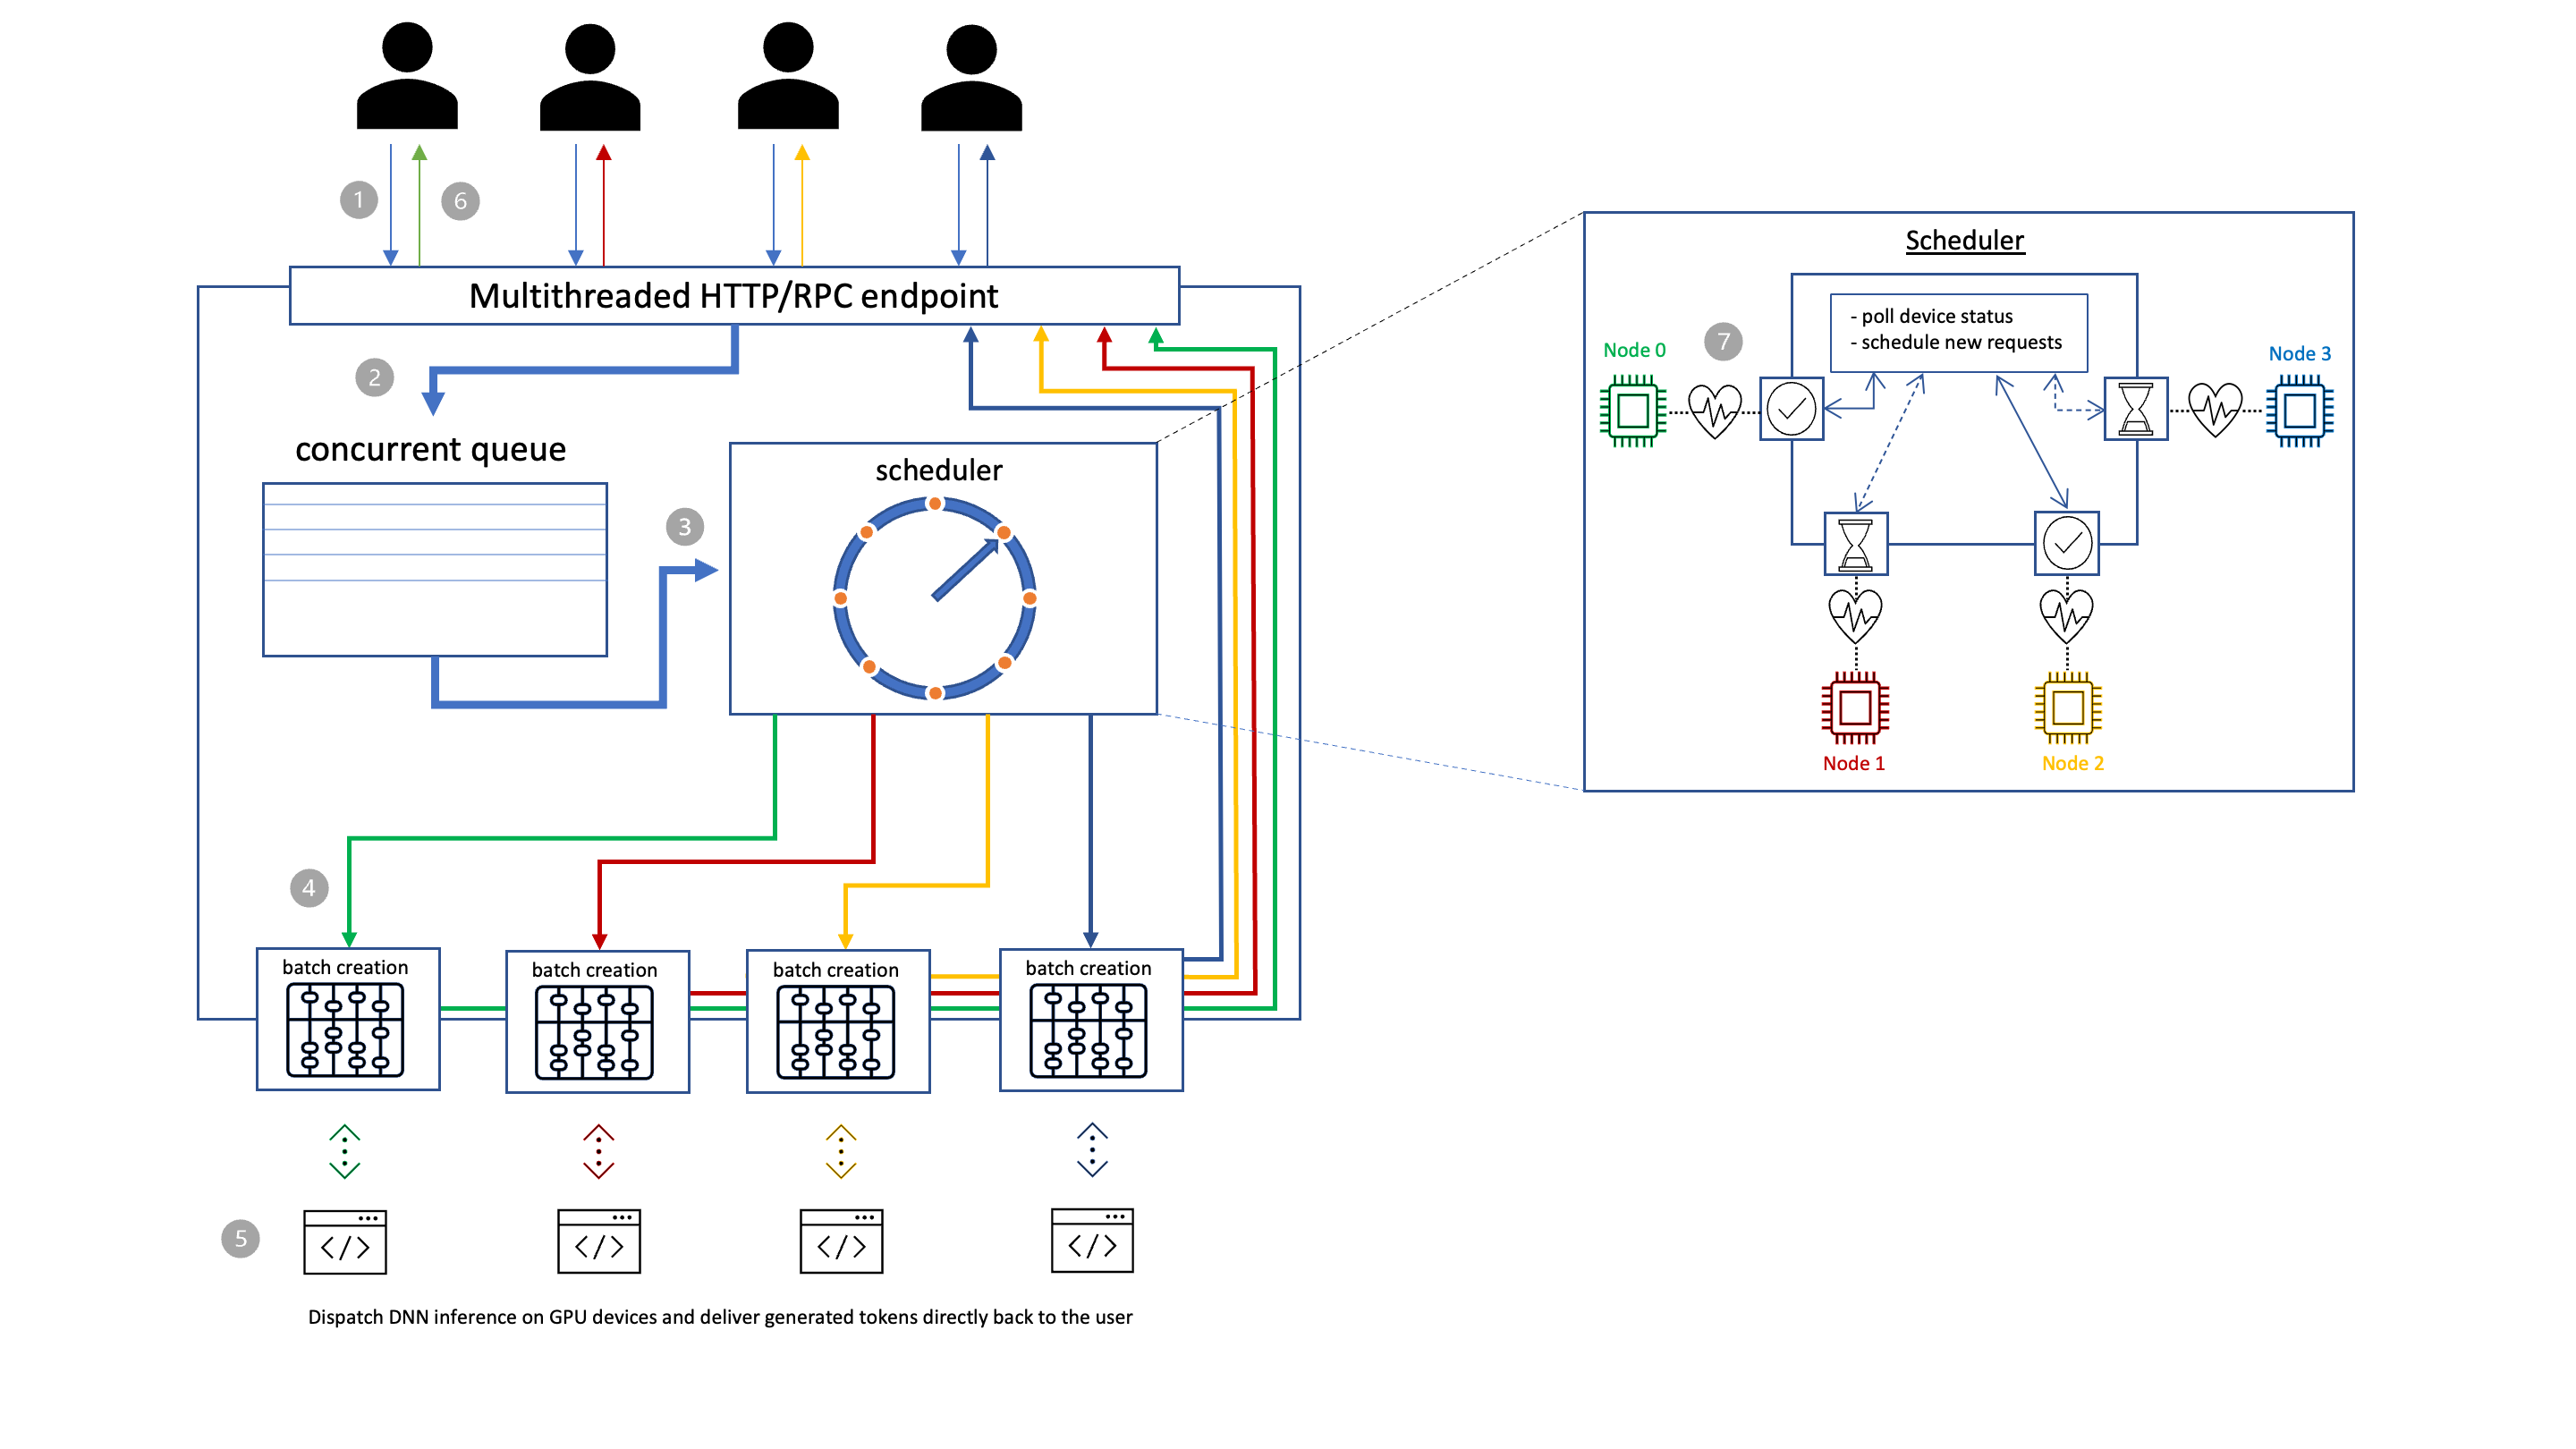
\includegraphics[width=\linewidth]{figures/design_illustration.png}
    }
    \caption{\textbf{The \Project system}}
    \label{fig:main-design-figure}
\end{figure}

The \Project frontend consists of an interactive interface, through which the user can submit a request \circled{1} by typing a prompt in a text box and pressing the submit button. The request is transmitted to the \Project server via HTTP or RPC, and received by a multithreaded server that is able to handle multiple requests from multiple users simultaneously. As they are received, the requests are stored in a high-speed lock-free concurrent queue \circled{2}, where they wait for their turn to be processed. The following steps in each request's journey through the \Project system are determined by the scheduler \circled{3}. When \Project is running, the scheduler polls each GPU node on the cluster to determine the current load, and dispatches requests to the first available node in round-robin fashion. After a request is assigned to a GPU, it will be routed to the corresponding Batch Manager \circled{4}, which is responsible for copying the request's tokens onto the model's input tensor, and updating the tensor metadata. Once the batch is ready, the runtime uses the FlexFlow~\cite{flexflow, unity} API to launch the asynchronous tasks \circled{5} that allow us to execute the DNN model. Once each iteration completes, the generated tokens are immediately returned to the original users \circled{6}. Note that while in the illustration above, for the sake of simplicity, each batch contains requests from a distinct user, batches generally contain requests from many different users at a time. The requests do not need to have the same length, nor to be at the same generation phase (e.g. at a given iteration, in a batch, a request may be in the process of generating token \#5, while another request may be generating token \#9). After each iteration has completed, if more requests are present in the queue, the scheduler \circled{7} will work together with the Batch Manager to add to the batch as many such requests as can fit while retaining the generated tokens from existing requests that have not yet completed. After rearranging, the updated batch is again sent to the corresponding node for the next iteration.

\section{Parallelization and Communication}
\Project uses a combination of data, model and pipeline parallelism. A typical GPT-MoE model parallelized by \Project is shown in Figure \ref{fig:expertflow-gpt-moe}.
\begin{figure}[]
    \centering
    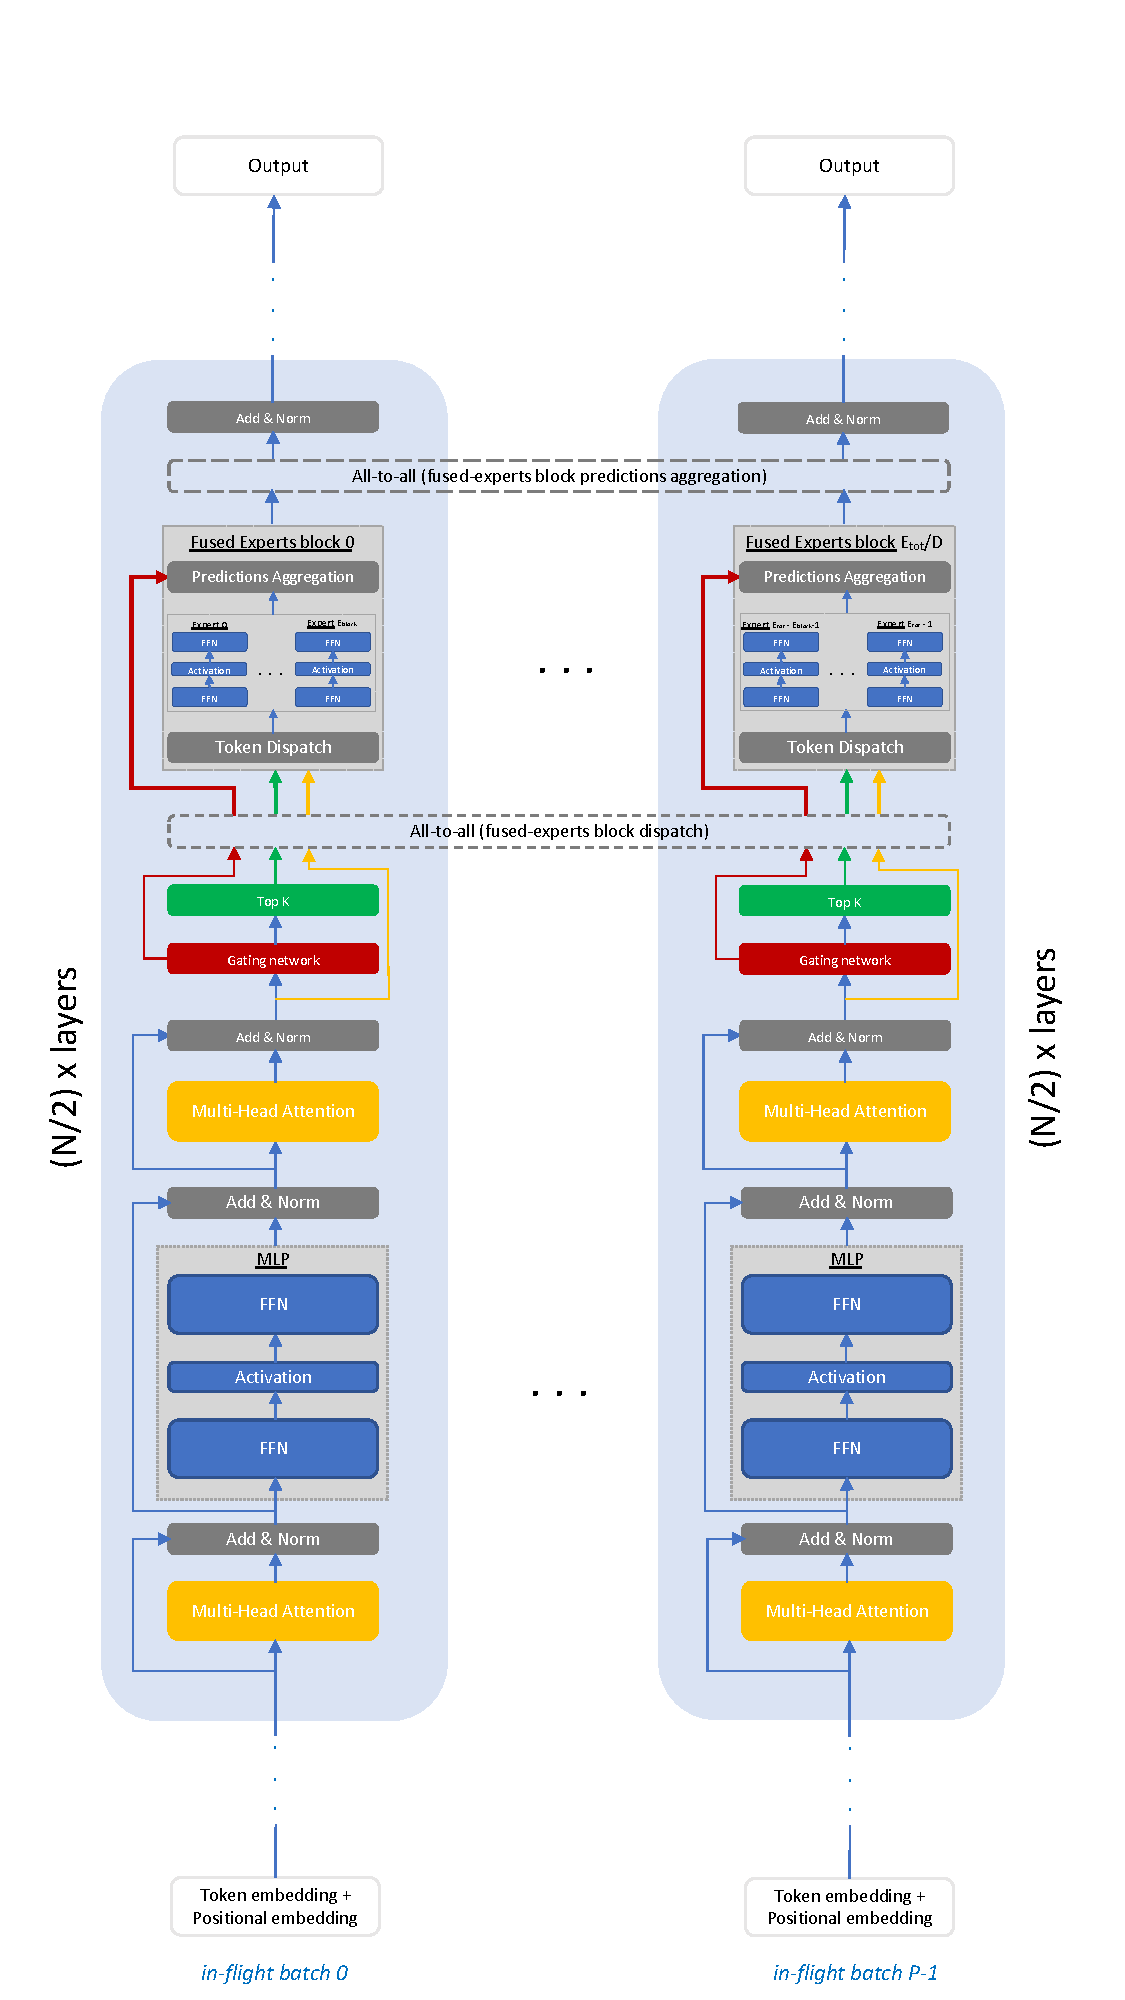
\includegraphics[width=0.9\linewidth]{figures/gpt-moe-illustration.pdf}
    \caption{\textbf{A typical GPT-MoE model parallelized in \Project}}
    \label{fig:expertflow-gpt-moe}
\end{figure}
The parallelization plan for a given machine is controlled by several parameters. In particular, the number of in-flight batches ($P$), the number of available devices ($D$), the number of experts ($E_{tot}$) and the desired size of each block of fused experts ($E_{block}$).

\textit{Data parallelism} is enabled whenever the number of in-flight batches is larger than 1 and the number of available GPUs is also greater than 1 (Equation \ref{eq:data_parallelism}). In this setup, up to $min(P, D)$ inflight batches are independently handled by a separate device, which will take care of both handling the data and running the model. The inflight batch is assigned to the device by the scheduler. 
\begin{equation}\label{eq:data_parallelism}
    \text{Data parallelism} \iff P > 1  \wedge D > 1
\end{equation}
\textit{Model parallelism} is enabled in two different scenarios. First of all, if the size of the model is larger than the memory available on any given GPU, we will be required to split the model's weight tensors across multiple GPUs, in tensor parallelism fashion. In addition, a particular form of model parallelism called \textit{expert parallelism} is available to the MoE layers in our models. Expert parallelism is activated whenever the condition in Equation \ref{eq:expert_parallelism} is met. Expert parallelism can be used for a similar reason as model parallelism: when the number of experts is significant (as is often the case), we may not be able to fit of all of them on a single device, so we can instead distributed them across the available nodes.
\begin{equation}\label{eq:expert_parallelism}
    \text{Expert parallelism} \iff E_{tot} > E_{block} \wedge D > 1
\end{equation}
Expert parallelism differs, however, from tensor parallelism in that each expert weight is not (necessarily) partitioned. Experts are sorted in groups, with $E_{block}$ experts in each block. The most naive sorting algorithm can simply assign experts to blocks using each expert's index, but more effective sorting will instead consider each expert's popularity (separating the most popular experts to avoid overwhelming a node), which can be estimated either offline or online. Unlike the training phase, the weights of the gating network, which effectively determine the distribution of the expert assignment function, do not change over time, so we can afford to use more static load balancing assignments. 
In addition to efficiently sorting the experts into blocks and placing the expert blocks on different devices, we also employ \textit{experts fusion} to increase the device utilization, especially under the smaller batch sizes that are typical in the inference phase. Expert fusion consists of fusing the computations from the experts in a block into a single kernel.
Finally, \textit{pipeline parallelism} allows us to run multiple stages of a model in parallel. This form of parallelism can be deployed manually by diving a model's layers in different stages and placing them on different GPUs. More commonly, pipeline parallelism can be done activated automatically as a consequence of the asynchronous execution of the model's inference tasks when Equation \ref{eq:pipeline_parallelism} holds, and especially when the number of CUDA streams is larger than 1.
\begin{equation}\label{eq:pipeline_parallelism}
    \text{pipeline parallelism} \implies P > D
\end{equation}


\section{Speculative Inference}
In order to further speed up the inference process when using large models, we support speculative inference, which allows us to to reduce the cost of token generation while leaving unchanged the quality of the output text. This is done by using two models of the same type, but different size. Usually, the bigger model has an order of magnitude more parameters than the smaller one. The inference procedure involves operating the small model in autoregressive mode for $\xi$ iterations, and then sending the resulting $\xi$ tokens as input to the larger model for verification. The larger model does not run in autoregressive mode, so a single iteration is enough for verifying all the tokens produced by the smaller model.